\documentclass[12pt]{article}
\usepackage[margin=1in]{geometry}
\usepackage{natbib}
\usepackage{hyperref}

\usepackage{listings}
\usepackage{rotating, graphicx}
\graphicspath{{./}, {./image/}}
\usepackage{booktabs, natbib}
% \usepackage{breakurl}
% \usepackage [english]{babel}
\usepackage{amsmath, amsbsy, amsthm, epsfig, epsf, psfrag, graphicx, 
amssymb, enumerate}
\usepackage{bm}
\usepackage{multirow, multicol}

\usepackage{color}
\definecolor{darkblue}{rgb}{0.1, 0.2, 0.6}
\usepackage{xcolor}
\newcommand{\jy}[1]{\textcolor{red}{JY: #1}}
\newcommand{\eds}[1]{\textcolor{blue}{(EDS: #1)}}
\newcommand{\mc}[1]{\textcolor{green}{(MC: #1)}}

\sloppy

% \usepackage{csquotes}
% \usepackage [autostyle, english = american]{csquotes}
% \MakeOuterQuote{"}

% \usepackage{bibentry}
\newenvironment{comment}%
{\begin{quotation}\noindent\small\it\color{darkblue}\ignorespaces%
}{\end{quotation}}


\begin{document}

\begin{center}
  {\Large\bf Response to the Comments}
\end{center}


% \jy{Spell check!}

\subsection*{Summary}

We thank the editor and the AE for the opportunity to revise the manuscript and
the two referees for their constructive comments. The manuscript has been
revised accordingly with the following notable changes:
\begin{enumerate}
\item 
  \begin{enumerate}
    \item 
    \item 
    \item 
    \item 
    \end{enumerate}
\item 
  \begin{enumerate}
  \item 
  \item 
  \item 
  \item 
  \end{enumerate}
\end{enumerate}



Point-by-point responses to the comments are as follows, with the
comments quoted in \emph{\color{darkblue} italic}.

\subsection*{To Referee 1}

\begin{comment}
1. It would be helpful to comment on the rationale for the proposed centered CI, 
especially in contrast to why a few others do not work for the log-1 
autocorrelation coefficient.
\end{comment}

\eds{Also added comment in the Recentered Percentile CI paragraph in the 
BLOCK BOOTSTRAP CIS section. Please check and add a comment here if you like it.}
\mc{looks good}

We have added this comment to the Recentered Percentile CI paragraph:
The motivation behind proposing such an interval was based on the 
simulation performance of the BC and BCA intervals, which will be discussed
further in the Results section. 

After discussion of the flaws of percentile, BC, and BCA CIs at the end of the
first paragraph of Discussion, we have included these additional comments on
why the proposed CI performs well:

The uncertainty measure from bootstrap, which is used to determine the width of
the percentile CI, is quite consistent in comparison to that used for BC and 
BCA CIs. However, for a percentile CI, the center seems
to be at the wrong location but is corrected when $\hat\theta_n$ is used as the
center. This is most likely the reason why the proposed recentered percentile CI
perfoms so much better than percentile, BC, and BCA CIs.

\begin{comment}
2. For all the figures, would it be possible to put the 6 figures in a column in 
a single plot? It would also be helpful to make the figures a bit larger. Right 
now it is hard to compare across different methods regarding their comparative 
performance.
\end{comment}

Below is an example of what this would look like. We find that it is a little
cluttered to make comparisons, so we will use the original format.

\begin{figure}[tbp]
  \centering
  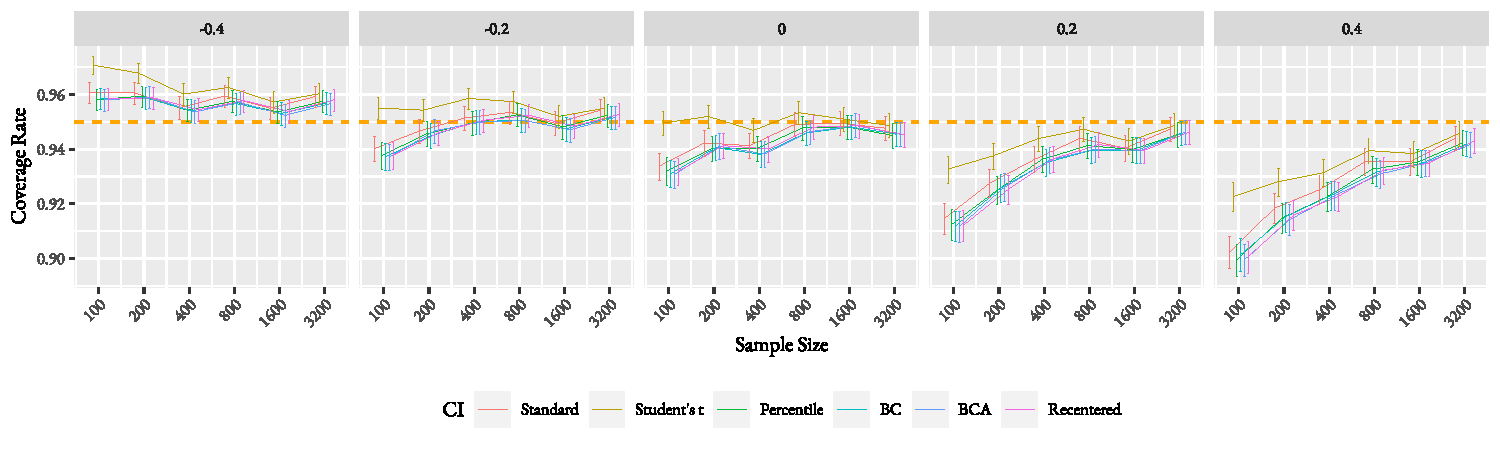
\includegraphics[width=\textwidth]{figures/alt_plot_norm_mu_1}
  \caption{Empirical coverage rates of different 95\% block bootstrap CIs for
    the marginal mean $\mu$ of an AR(1) process with a marginal standard 
    normal distribution with AR coefficient
    $\phi \in \{-0.4, 0.2, 0, 0.2, 0.4\}$ and series length
    $n \in \{100, 200, 400, 800, 1600, 3200\}$ based on 10,000 replicates. The
    error bars represent 95\% CIs of the real coverage rates.}
  \label{fig:mu}
\end{figure}




\begin{comment}
3. The Appendix should be moved to the main text? Assessing the performance of 
various CI formulations for non-normal error is of central interest.
\end{comment} 

The text from the Appendix has been moved to the Simulation Study 
section. The second reviewer suggested block size as an additional experimental
factor, so the paragraphs for normal and exponential error structures have
been adjusted accordingly.

\eds{I also added subsubsections (paragraphs) for the Normal and Exponential 
Marginal Distributions under Design and Results subsections.
Is it possible to put to make the [Simulation Study] Design and 
[Simulation Study] Results as two separate 
sections instead of placing each as subsections of the Simulation Study section,
or does the journal formatting prohibit this?  If you can change this, then the 
Normal and Exponential Marginal subsubsections can be updated to subsections
under the Simulation Study Design and Simulation Study Results sections.}  
\mc{addressed}


\begin{comment}
4. The authors might want to discuss in what circumstances “non-parametric” CI 
formulas would work better. It is a bit surprising that student’s t based 
formula works well under both normal and non-normal error structures.
\end{comment}

We have included this comment in the Exponential Marginal Distribution 
subsection of the Design section:

It is important to note that we expect the CIs that are based on bootstrap 
"tables" to depend on the 
asymptotic distribution of the statistics, but we expect such CIs to 
have similar performance for different error structures. For example, under the 
Central
Limit Theorem, we expect the asymptotic distribution of the sample mean to be 
approximately 
normal for both marginal normal distributions and marginal exponential 
distributions. Therefore, we do not expect CIs that are not based on bootstrap
"tables" (Percentile, BC, BCA, Recentered Percentile CI) to perform better under
non-normal error structures.
\eds{you will need to add more here.  This concerns the
(asymptotic) distribution of the statistics, not the underlying error 
structure.}
\mc{I changed it a bit... I'm not sure what to say for circumstances in which
“non-parametric” CI 
formulas would work better}


\begin{comment}
5. Page 3, 2nd line after “Standard Normal CI”: “p.168” does not seem to fit?
\end{comment}

Because of the style constraints for AJUR, we have removed page numbers in 
citations.

\subsection*{To Referee 2}

\begin{comment}
1. The authors say “....the standard CI is a table-based bootstrap…..”.  
What is meant by “table-based” here?  Is this just a reference to how critical 
values used to be listed in tables?  If that’s the case, I wouldn’t refer to 
this as a “table-based” interval. 
\end{comment}

Thank you for the comment.  This terminology was used because 
\citet{efron1993introduction} refers to such CIs as 
"confidence intervals based on 
bootstrap 'tables'." We have changed these sentences as shown below:

The standard CI is classified by \citet{efron1993introduction} 
as a confidence interval based on bootstrap "tables".
Like the standard normal interval, the
Student's $t$ CI is classified by \citet{efron1993introduction} 
as a confidence interval based on bootstrap "tables".


\begin{comment}
2. Just a comment: The recentered percentile CI proposed here is an interesting 
interval to study. 
\end{comment}

We agree. We have added this comment to the discussion:

Lastly, because of its exceptional performance in comparison to the other 
CIs that are not based on bootstrap "tables", the proposed recentered percentile 
CI would be
an interesting method to study further with different bootstrap schemes.

\begin{comment}
3. The sections are numbered, which makes it awkward when the authors refer back 
to a section.  For instance, they refer to “...procedures described in Block 
Bootstrap CIS.”  This would be easier to refer to if the sections were numbered.  
(Is this a journal style choice?  If so, then you can ignore this comment.)
\end{comment}

This is a journal style choice.

\begin{comment}
4.  In Figure 1 (and all the other figures), the authors present confidence 
intervals for the real coverage rates.  The authors should specify what type of 
CI they are using here.  I assume the authors are using a Wald-type interval for 
this CI as this is for a proportion.  If that’s the case, it’s well known that 
the Wald-type interval has undercoverage when the true proportion is near 0 or 
1, which is the case in several of these scenarios, especially when phi is -0.4. 
\end{comment}

We modified the Design section as below:

Because it is unlikely for the coverage to 
exactly match the nominal level, we can construct a 95\% Wald-type CI of the 
coverage rate 
(which is an estimate of a proportion with $R = 10000$). If the proportion 0.95 
is included in the interval, the block bootstrap method is likely performing 
well. If all values in the interval are below 0.95, the results would suggest 
that the method either is providing inaccurate estimation, is underestimating 
the process' variability, or a combination of both. If all values in the 
interval are above .95, the results suggest that the method is overestimating 
the process' variability. \citet{brown2001interval} notes that the Wald-type 
interval has poor coverage as the proportion approaches 0 or 1.

\eds{I don't think this answers the question.  The reviewer is saying that 0.95 
is close to the boundary of 1, so the undercoverage observed intervals
(especially when phi -0.4) may be due, at least in part, to the flaws 
of the asymptotic Wald interval you are using. 
\@ Jun: do you think he should try exact Clopper-Pearson
intervals for at least a few cases of undercoverage to verify it is not the Wald
interval that is causing the undercoverage, then comment on this in at least the
reply (and possibly also in the main paper)?}
\mc{plot_norm_mu_1_cup.pdf (exact Clopper-Pearson) seems to have about the same 
widths for high 
proportions
(especially for phi = -0.4) as plot_norm_mu_1.pdf (Wald-Type)}


\begin{comment}
5.  In all the figures, the y-axis is allowed to vary freely making it hard to 
compare one row directly to another.  I would suggest fixing the limits on the 
y-axis to make comparisons easier.  
\end{comment}

Because of the deterioration for $\phi$, we found it hard to fix the limits on 
the 
y-axis without hurting the visualization for the other rows. 
Figure~\ref{fig:alt_phi1} is an 
example:  \eds{refer to the Figure label, and avoid using `below' and `above'
terminology with latex because the figures are not always positioned as we may
have intended.}
\mc{addressed}

\begin{figure}[tbp]
  \centering
  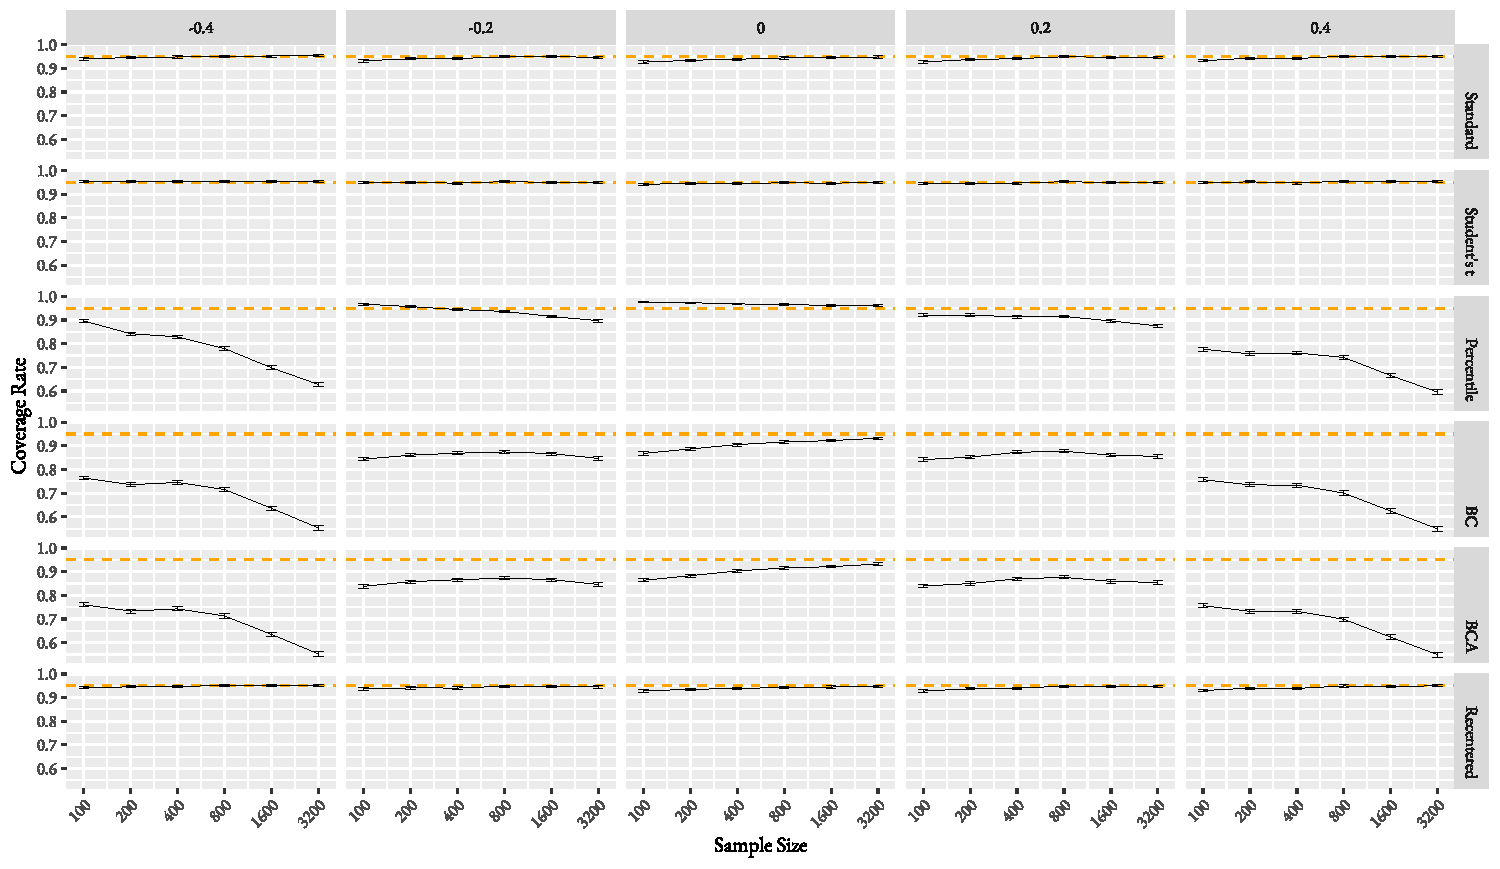
\includegraphics[width=\textwidth]{figures/alt2plot_norm_phi_1}
  \caption{Empirical coverage rates of different 95\% block bootstrap CIs for 
    the first-order autocorrelation coefficient $\phi$ of an AR(1) process with 
    a marginal standard normal distribution with 
    $\phi \in \{-0.4, 0.2, 0, 0.2, 0.4\}$ and series length
    $n \in \{100, 200, 400, 800, 1600, 3200\}$ based on 10,000 replicates of
    block bootstrap with $l = \lceil n^{1/3} \rceil$. The
    error bars represent 95\% CIs of the real coverage rates.}
  \label{fig:alt_phi1}
\end{figure}

\begin{comment}
6.  Is there a reason why the coverage for mu (in Figure 1) is better for 
negative autoregressive terms when compared with the positive autoregressive 
term? Can the authors give some intuition behind why that makes sense? 
\end{comment}

We have included this comment at the end of the paragraph on estimation of 
$\mu$:

A possible explanation for this is that if a 
stationary series has a positive 
autocorrelation, the effective sample
size is decreased, whereas is a series has a negative autocorrelation, the
effective sample size is increased. Additionally, this seems to have a 
greater effect on the the estimation of the location parameter versus that
of the scale parameter or temporal dependence parameter.

\begin{comment}
7.  The authors say “A smaller sample size is generally required to estimate a 
parameter for a sample with a negative phi versus a positive phi of the same 
magnitude.”  On a quick reading of this it sounds like the authors are 
recommending using a smaller sample size when phi is negative.  I believe what 
you are trying to say is that coverage rates are acceptable at smaller sample 
sizes when phi is negative versus when phi is positive (i.e. it takes larger 
sample sizes to get acceptable coverage when phi is positive).  Change this 
sentence to make it more clear. 
\end{comment}

Thank you for pointing this out. The original sentence has been replaced 
with:

Coverage rates are acceptable at smaller sample 
sizes when phi is positive versus when phi is negative. In
other words, a larger sample size is generally required to estimate a 
parameter for a sample with a negative $\phi$ versus a positive $\phi$ of the 
same magnitude.

\begin{comment}
8.   In the Discussion section, the authors say “We know theoretically that the 
block bootstrap procedure will cover the parameter of a time series given an 
infinitely large sample.”  Essentially, you are stating that the estimator is 
consistent.  Is there a citation that you can point to that shows that this is 
true? 
\end{comment}

\citep{calhoun2018} 

\eds{I only saw this citation in the abstract, not the discussion.  
Please remove this citation from the abstract and place in the discussion 
section where the sentence in question appears. In general,
try to avoid placing any citations in the abstract.}
\mc{addressed, sorry silly mistake}

\begin{comment}
9.   The authors studied coverage rates of the different intervals as a function 
of sample size, but they only looked at one choice for the number of blocks.  
Why did the authors choose to not also look at how the number of blocks affects 
the coverage rates?
\end{comment}

We have now repeated the same simulation study with block size as an 
additional experimental factor. The optimal order of block size is 
$\lceil n^{1/3} \rceil$, so we tried the same simulations using 
$l = \lceil n^{1/3} \rceil$ and $l = \lceil 2n^{1/3} \rceil$. We have included
the changed Results subsection below:

\eds{\@ Jun: what do you think about putting the $l = \lceil 2n^{1/3} \rceil$
results in the Appendix, but keeping the conclusions regarding how the 
$l = \lceil n^{1/3} \rceil$ and $l = \lceil 2n^{1/3} \rceil$ simulations differ
in the main text?}

\begin{figure}[tbp]
  \centering
  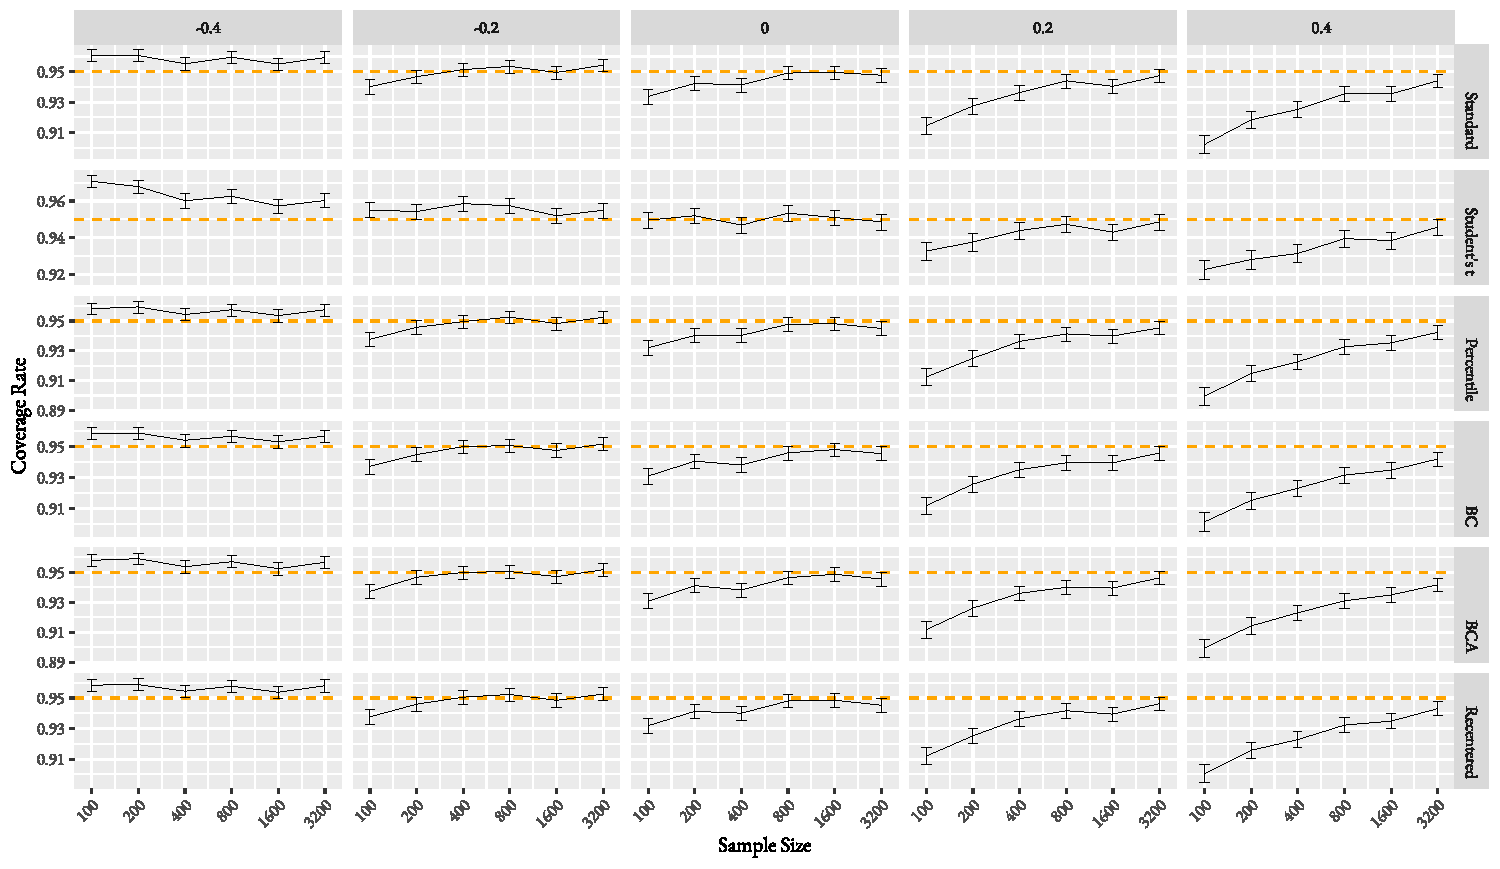
\includegraphics[width=\textwidth]{figures/plot_norm_mu_1}
  \caption{Empirical coverage rates of different 95\% block bootstrap CIs for
    the marginal mean $\mu$ of an AR(1) process with a marginal standard 
    normal distribution with AR coefficient
    $\phi \in \{-0.4, 0.2, 0, 0.2, 0.4\}$ and series length
    $n \in \{100, 200, 400, 800, 1600, 3200\}$ based on 10,000 replicates of
    block bootstrap with $l = \lceil n^{1/3} \rceil$. The
    error bars represent 95\% CIs of the real coverage rates.}
  \label{fig:mu1}
\end{figure}


\begin{figure}[bp]
  \centering
  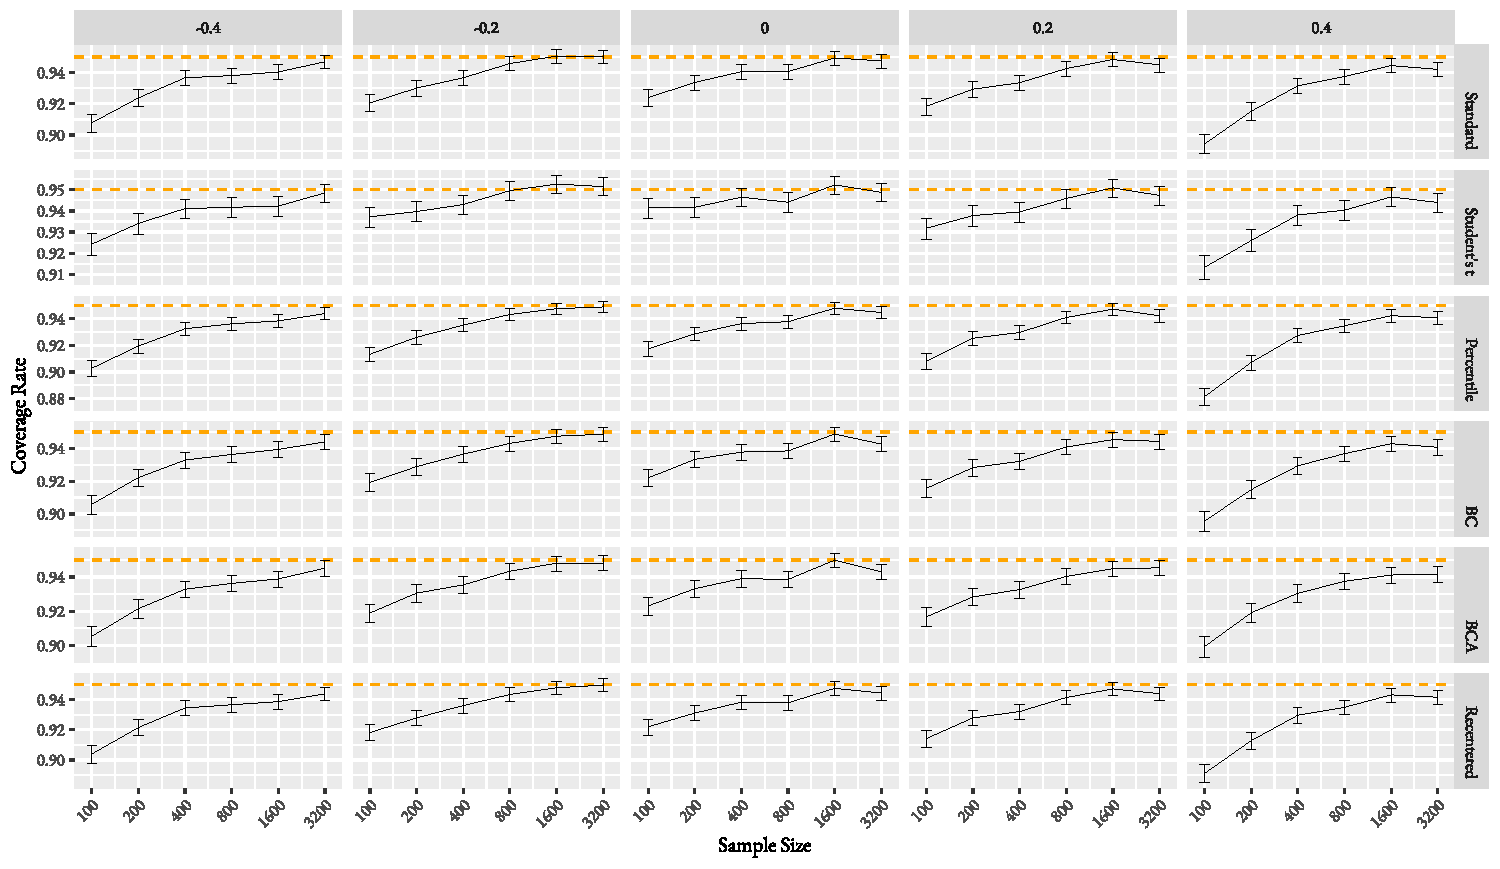
\includegraphics[width=\textwidth]{figures/plot_norm_sigma_1}
  \caption{Empirical coverage rates of different 95\% block bootstrap CIs for
    the marginal standard deviation $\sigma_x$ of an AR(1) process with a
    marginal standard normal distribution with AR 
    coefficient $\phi \in \{-0.4, 0.2, 0, 0.2, 0.4\}$ and series length 
    $n \in \{100, 200, 400, 800, 1600, 3200\}$ based on 10,000 replicates of
    block bootstrap with $l = \lceil n^{1/3} \rceil$. The 
    error bars represent 95\% CIs of the real coverage rates.}
  \label{fig:sigma1}
\end{figure}


\begin{figure}[tbp]
  \centering
  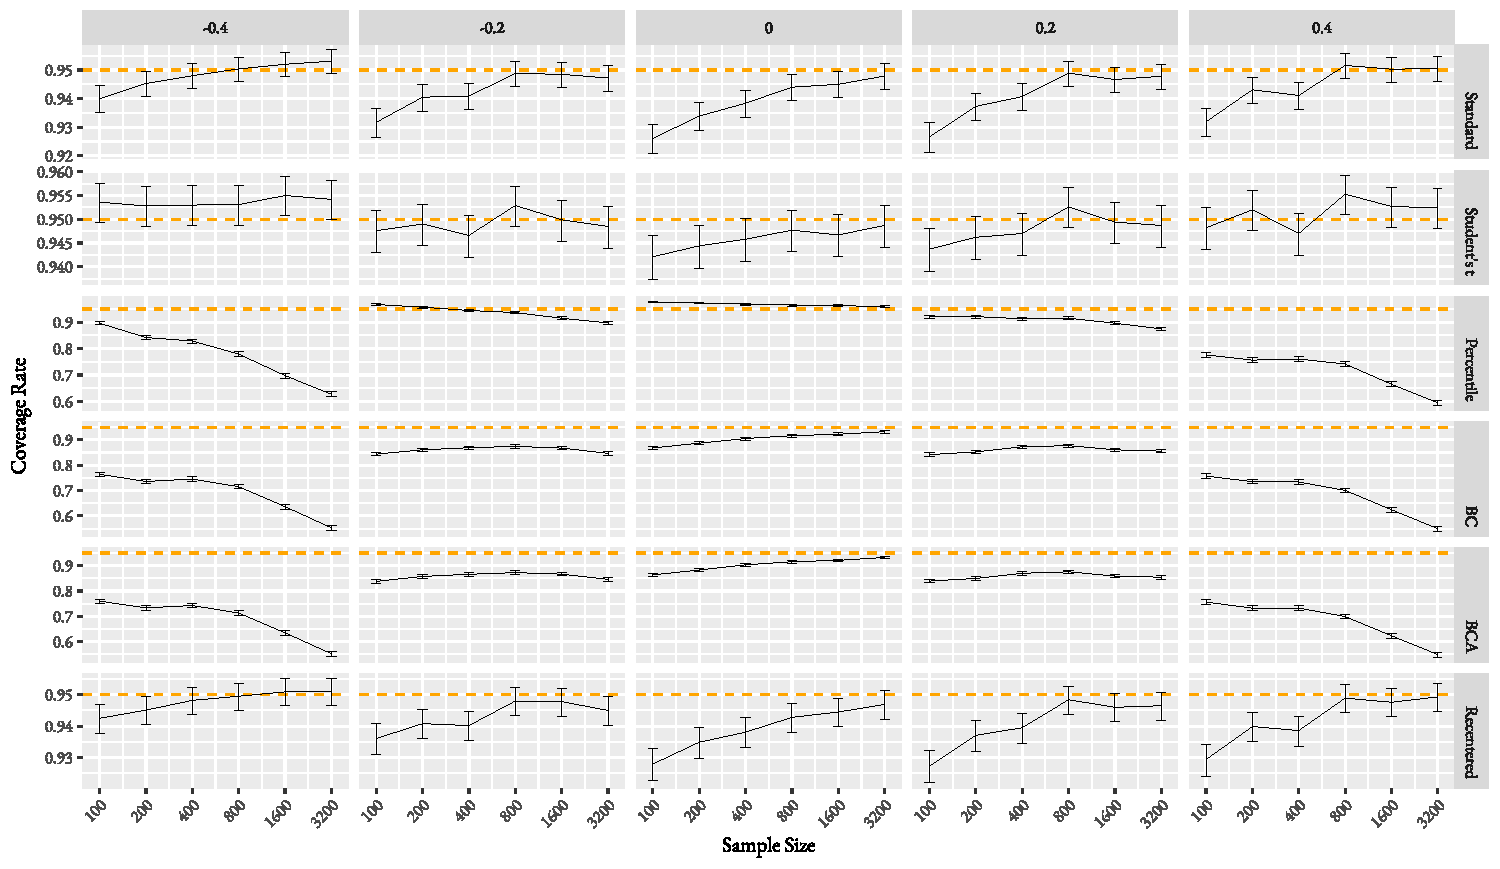
\includegraphics[width=\textwidth]{figures/plot_norm_phi_1}
  \caption{Empirical coverage rates of different 95\% block bootstrap CIs for 
    the first-order autocorrelation coefficient $\phi$ of an AR(1) process with 
    a marginal standard normal distribution with 
    $\phi \in \{-0.4, 0.2, 0, 0.2, 0.4\}$ and series length
    $n \in \{100, 200, 400, 800, 1600, 3200\}$ based on 10,000 replicates of
    block bootstrap with $l = \lceil n^{1/3} \rceil$. The
    error bars represent 95\% CIs of the real coverage rates.}
  \label{fig:phi1}
\end{figure}


\begin{figure}[tbp]
  \centering
  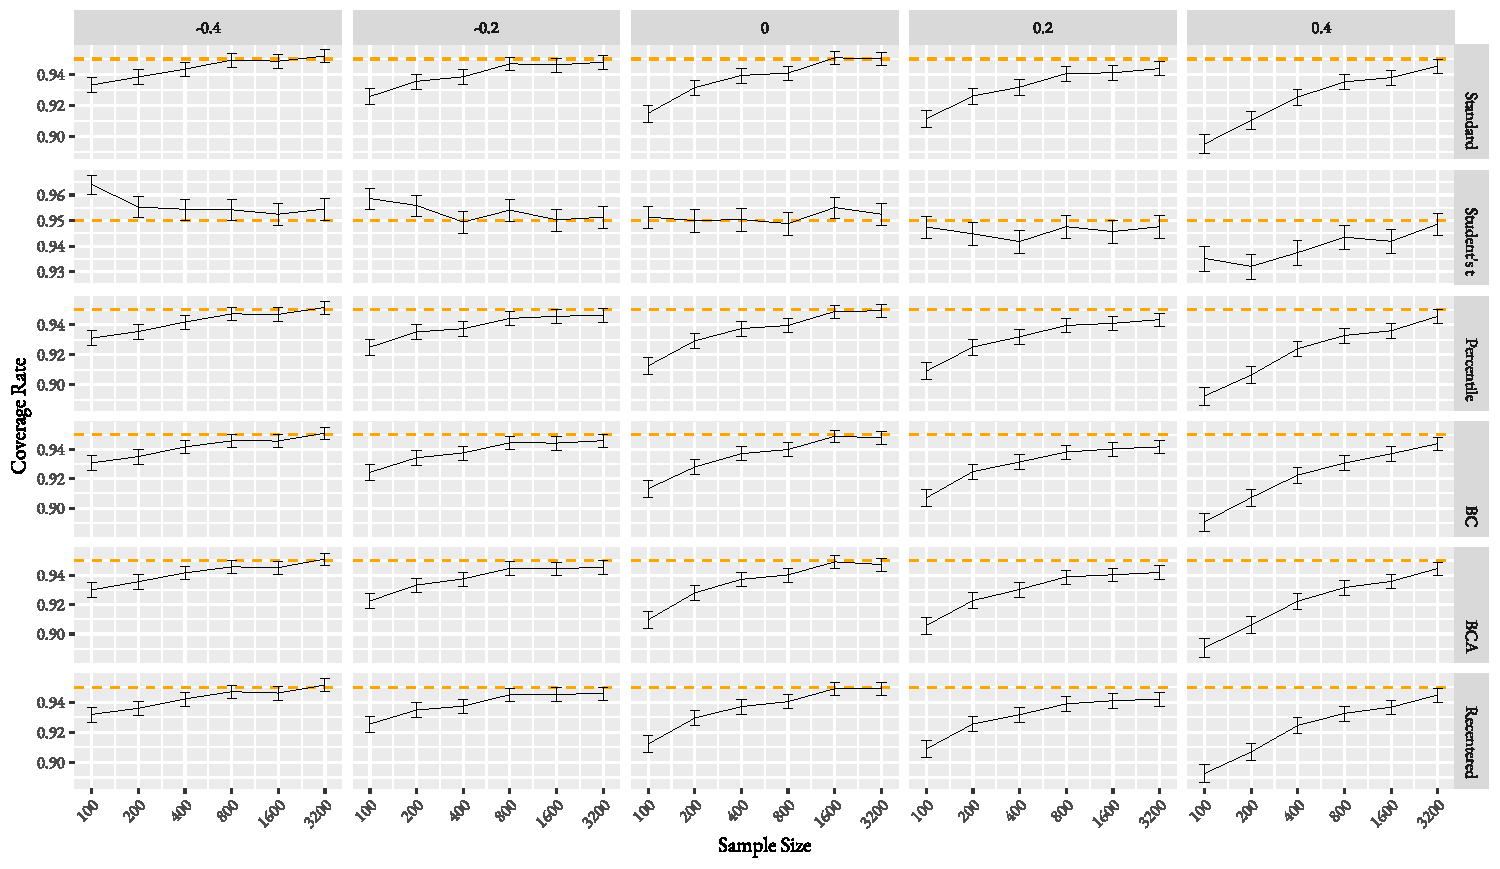
\includegraphics[width=\textwidth]{figures/plot_norm_mu_2}
  \caption{Empirical coverage rates of different 95\% block bootstrap CIs for
    the marginal mean $\mu$ of an AR(1) process with a marginal standard 
    normal distribution with AR coefficient
    $\phi \in \{-0.4, 0.2, 0, 0.2, 0.4\}$ and series length
    $n \in \{100, 200, 400, 800, 1600, 3200\}$ based on 10,000 replicates of
    block bootstrap with $l = \lceil 2n^{1/3} \rceil$. The
    error bars represent 95\% CIs of the real coverage rates.}
  \label{fig:mu2}
\end{figure}


\begin{figure}[bp]
  \centering
  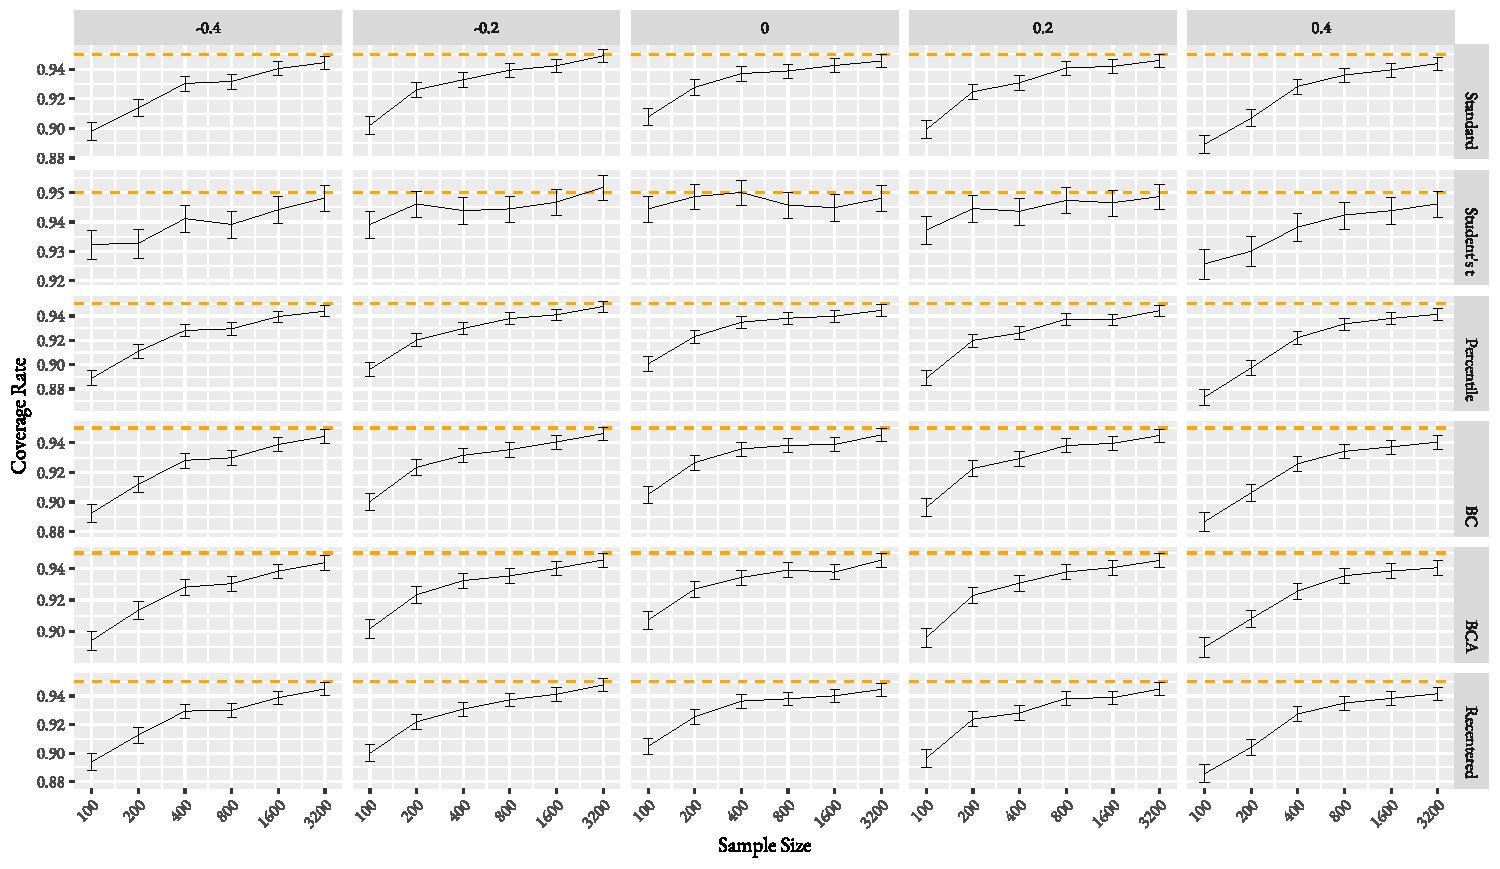
\includegraphics[width=\textwidth]{figures/plot_norm_sigma_2}
  \caption{Empirical coverage rates of different 95\% block bootstrap CIs for
    the marginal standard deviation $\sigma_x$ of an AR(1) process with a
    marginal standard normal distribution with AR 
    coefficient $\phi \in \{-0.4, 0.2, 0, 0.2, 0.4\}$ and series length 
    $n \in \{100, 200, 400, 800, 1600, 3200\}$ based on 10,000 replicates of
    block bootstrap with $l = \lceil 2n^{1/3} \rceil$. The 
    error bars represent 95\% CIs of the real coverage rates.}
  \label{fig:sigma2}
\end{figure}


\begin{figure}[tbp]
  \centering
  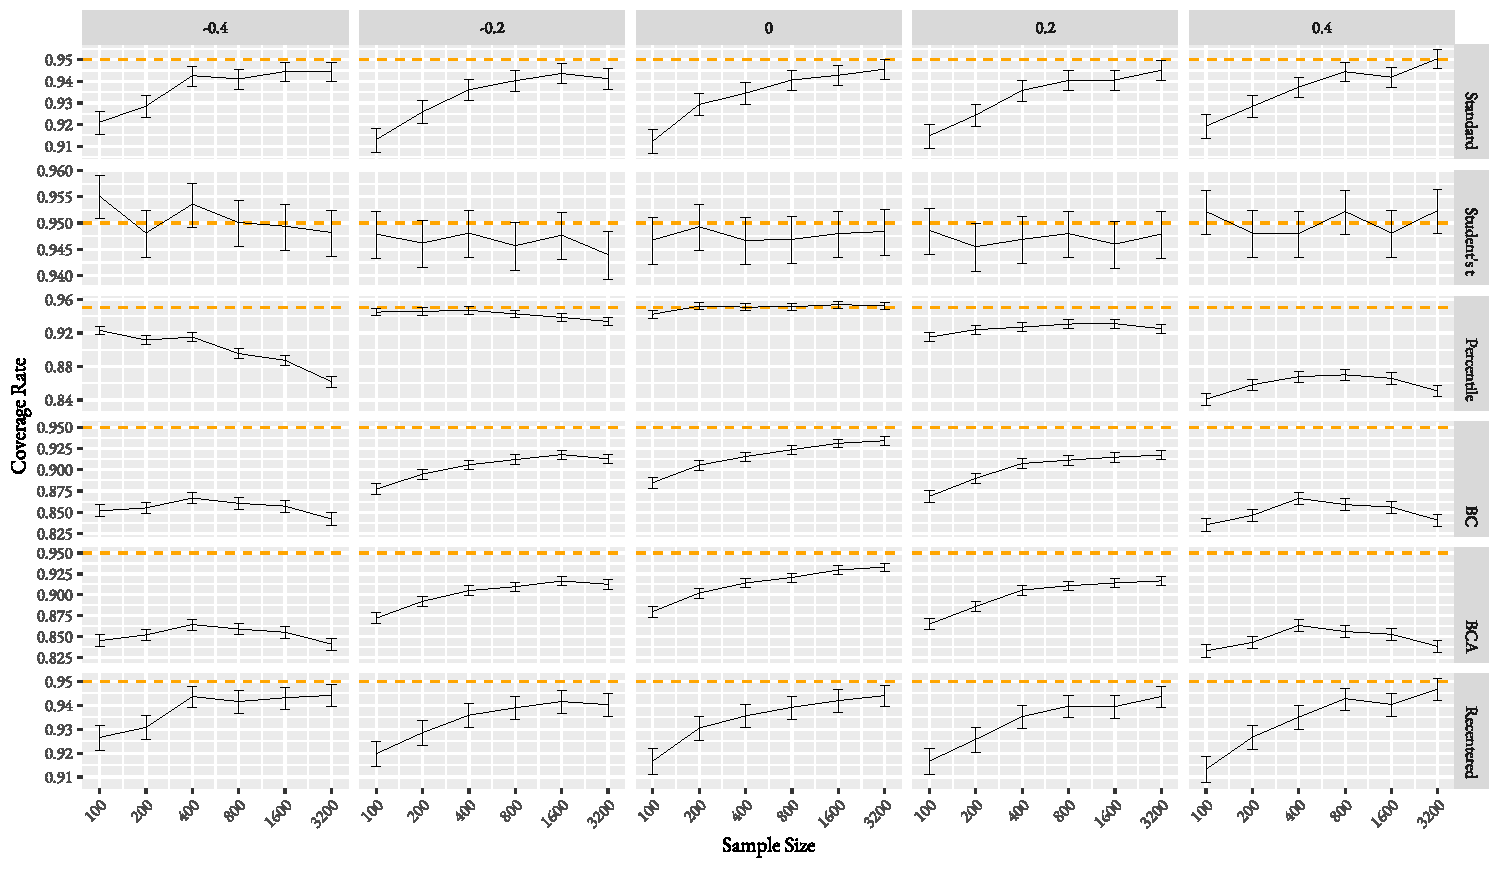
\includegraphics[width=\textwidth]{figures/plot_norm_phi_2}
  \caption{Empirical coverage rates of different 95\% block bootstrap CIs for 
    the first-order autocorrelation coefficient $\phi$ of an AR(1) process with 
    a marginal standard normal distribution with 
    $\phi \in \{-0.4, 0.2, 0, 0.2, 0.4\}$ and series length
    $n \in \{100, 200, 400, 800, 1600, 3200\}$ based on 10,000 replicates of
    block bootstrap with $l = \lceil 2n^{1/3} \rceil$. The
    error bars represent 95\% CIs of the real coverage rates.}
  \label{fig:phi2}
\end{figure}


For estimating the mean parameter~$\mu$, \textbf{Figure~\ref{fig:mu1}} suggests 
that all methods eventually approach correct coverage of $\mu$ as sample size 
increases. Student's $t$ CIs appear to need the smallest sample size to achieve 
correct coverage, except for samples with strong negative dependence, in which 
case, they actually over-cover $\mu$ for smaller sample sizes. For instance, for 
a sample with $n = 100$ and $\phi = -0.4$, the lower bound for a Students $t$ 
CI's coverage of $\mu$ is greater than 95\%, whereas the coverage intervals for 
other methods contain 95\%. The standard normal, percentile, BC, and BCA, and 
recentered percentile CIs require similar sample sizes to recover $\mu$ at the 
nominal level for all combinations of $n$ and $\phi$. All methods seem to 
require a smaller sample to recover $\mu$ at the nominal rate when dealing with 
negative dependence versus positive dependence. For example, BC CIs recover 
$\mu$ for $n \geq 100$ when $\phi = -0.2$, but they only recover $\mu$ for 
$n \geq 800$ when $\phi = 0.2$. In addition, as a negative dependence gets 
stronger, holding everything else equal, coverage increases, which lead to the 
Student $t$ CI's aforementioned over-coverage. As a positive dependence gets 
stronger, holding everything else equal, coverage decreases, and a larger sample 
is necessary to recover~$\mu$.  A possible explanation for this is that if a 
stationary series has a positive 
autocorrelation, the effective sample
size is decreased, whereas is a series has a negative autocorrelation, the
effective sample size is increased. Additionally, this seems to have a 
greater effect on the the estimation of the location parameter versus that
of the scale parameter or temporal dependence parameter.


For estimating the standard deviation parameter~$\sigma_x$,
\textbf{Figure~\ref{fig:sigma1}} suggests that every method can reach nominal 
coverage of $\sigma_x$ if the sample is large enough, but for a given $n$ and 
$\phi$, coverage of $\sigma_x$ will be lower than coverage of $\mu$ in general.
Like $\mu$, $\sigma_x$ can be covered by Student $t$ CIs with smaller sample 
sizes when compared to other methods. Unlike $\mu$, there is no over-coverage 
issue for $\sigma_x$ when $\phi = -0.4$. Standard normal, percentile, BC, BCA, and 
recentered percentile CIs again have similar performance. All methods seem to 
have slightly higher coverage of $\sigma_x$ when $\phi$ is negative versus when 
$\phi$ is positive. Regardless of the sign, coverage of $\sigma_x$ gets worse as 
the strength of the temporal dependence increases.


For estimating the autocorrelation parameter~$\phi$, 
\textbf{Figure~\ref{fig:phi1}} suggests that while standard normal, Student's $t$, and 
recentered percentile CIs do approach correct coverage as sample size increases, 
percentile, BC, and BCA CIs deteriorate as sample size increases, especially as 
the strength of the temporal dependence increases. Because of this, only 
standard normal, Student's $t$, and recentered percentile CIs should be considered as 
effective block bootstrap methods to estimate $\phi$. Student's $t$ CIs once 
again can achieve correct coverage with smaller sample sizes when compared to 
standard and recentered percentile CIs which perform similarly. Student's $t$ 
CIs can can recover $\phi$ at the nominal level for $n \geq 100$ when the 
sample's temporal dependence is as strong as 0.4. Coverage appears to be higher 
for all methods when the dependence is negative rather than positive. Whether or 
not the dependence is negative or positive, coverage of $\phi$ seems to increase 
slightly as the absolute value increases for standard normal, Student's $t$, and 
recentered percentile CIs. For the values of $\phi$ observed, there are no 
examples of over-coverage for standard normal, Student's $t$, BC, BCA, or recentered 
percentile CIs. However, percentile CIs appear to over-cover $\phi$ for smaller 
sample sizes when $\phi = -0.2$ and when $\phi = 0$, indicating again that they 
should not be used.

Based on \textbf{Figure~\ref{fig:mu2}}, for negative autocorrelations, the 
coverage 
rates of $\mu$ appear to be lower when
using $l = \lceil 2n^{1/3} \rceil$. For example, whereas $n = 100$ or 200 
would seem sufficient for most CIs when using $l = \lceil n^{1/3} \rceil$, 
$n = 800$ or 1600 is necessary to capture negative autocorrelations for 
$l = \lceil n^{1/3} \rceil$. Student's $t$ CIs do not seem to be as affected
by this change in $l$: for $\phi = -0.4$ and -0.2, they still overcover $\mu$
for smaller values of $n$. 

\textbf{Figure~\ref{fig:sigma2}} looks very similar to 
\textbf{Figure~\ref{fig:sigma1}}, but coverage rates of $\sigma$ do look 
slightly lower
especially for negative values of $\phi$, although Student's $t$ CIs are again
not as influenced by this change in $l$. A larger sample size seems necessary
when using other CIs to estimate $\sigma$ for $l = \lceil 2n^{1/3} \rceil$.

As shown in \textbf{Figure~\ref{fig:phi2}},
recentered percentile and standard CIs have slightly lower coverage rates when
estimating negative values of $\phi$ with $l = \lceil 2n^{1/3} \rceil$. 
Although it is still a problem, the coverage deterioration appears to be less 
dramatic for BCA,
BC, and percentile CIs.

Aside from these differences, the overall changes
in performance when other experimental factors are changed are the same.

\begin{figure}[tbp]
  \centering
  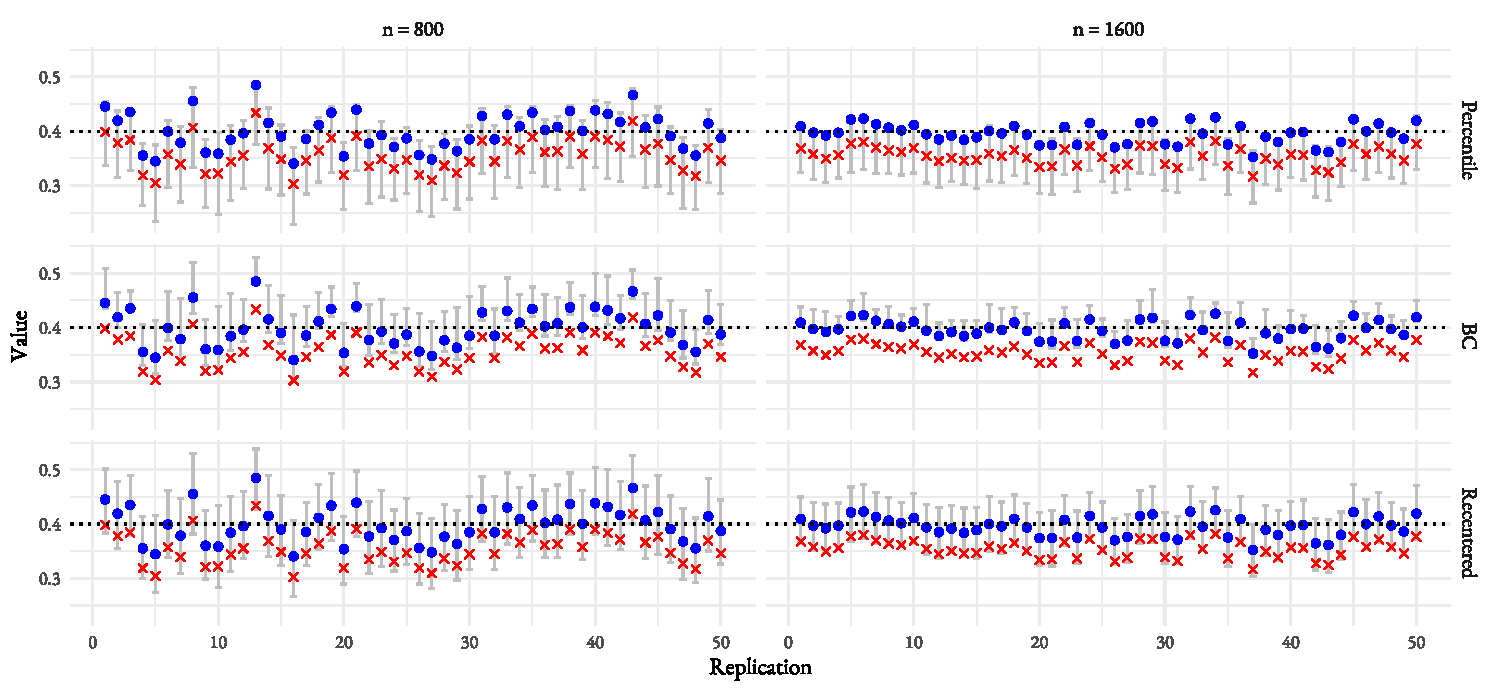
\includegraphics[width=\textwidth]{figures/norm_phi_intervals}
  \caption{50 replicate percentile, BC, and recentered percentile CIs for 
    samples of $n \in \{800, 1600\}$ ($l = \lceil n^{1/3} \rceil$)
    for an AR(1) process with $\phi = 0.4$. For 
    each replicate, the lower and upper bounds of the CIs are displayed, as well 
    as $\hat\theta_n$ (blue circle) and $\bar\theta_n^{B}$ (red cross).}
  \label{fig:npi}
\end{figure}


The outcomes of the $\phi$ estimation raise a natural question about the 
lackluster performance of certain methodologies. To delve into this inquiry, a
set of 50 CIs was generated for each of the percentile, BC, and recentered
percentile  approaches for samples of $n \in \{800, 1600\}$. Illustrated in 
\textbf{Figure~\ref{fig:npi}}, it becomes evident that the percentile-based CIs 
exhibit a notable bias, predominantly manifesting as a substantial 
underestimation of $\phi$ with point estimator $\bar\theta_n^B$, that is, the 
average of $B$ bootstrap point estimates. As the sample size increases from 800 
to 1600, this bias does not vanish while the uncertainty reduces, which explains 
why the coverage rates deteriorate. The bias in $\bar\theta_n^B$ also appears to 
invalidate the bias-correction in the BC bootstrap, leading to the poor 
performance of the BC intervals. The BCA intervals have the same problem as the 
BC intervals in the bias-correction step. The root of the issue appears to be 
that the autocorrelation in the block bootstrap samples is somehow smaller 
compared to that in the original sample. On the other hand, the original point 
estimator $\hat\theta_n$ is asymptotically unbiased. Since the width is based on 
the uncertainty in the bootstrap point estimates $\hat\theta_n^{(b)}$, 
$b = 1, \ldots, B$, the percentile CIs recentered at the original point estimate
$\hat\theta_n$ provide desired coverage.


To summarize, the performance of the CIs depends on the target parameter. When
estimating $\mu$ and $\sigma_x$, any CI will do, although Student's $t$ CIs
perform noticeably better than the others.
However, when estimating $\phi$, the 
choice of method is of utmost importance as to avoid coverage deterioration. 
In addition, choice of block size is another important parameter, as
$l = \lceil n^{1/3} \rceil$ results in better coverage than 
$l = \lceil 2n^{1/3} \rceil$.
Coverage rates are acceptable at smaller sample 
sizes when phi is positive versus when phi is negative. In
other words, a larger sample size is generally required to estimate a 
parameter for a sample with a negative $\phi$ versus a positive $\phi$ of the 
same magnitude. In order 
to know if coverage will increase as the strength of the temporal dependence 
increases, one need to know what the parameter of interest is, and in the case 
of $\mu$, the direction of the serial dependence. The BC approach does not seem 
to be correcting bias appropriately when estimating $\phi$. Like the percentile 
method, the recentered percentile method uses the spread from the bootstrap to 
construct the width of the CI. However, the recentered approach, does not 
correct from the original point estimate $\hat\theta_n$.


\begin{figure}[tbp]
  \centering
  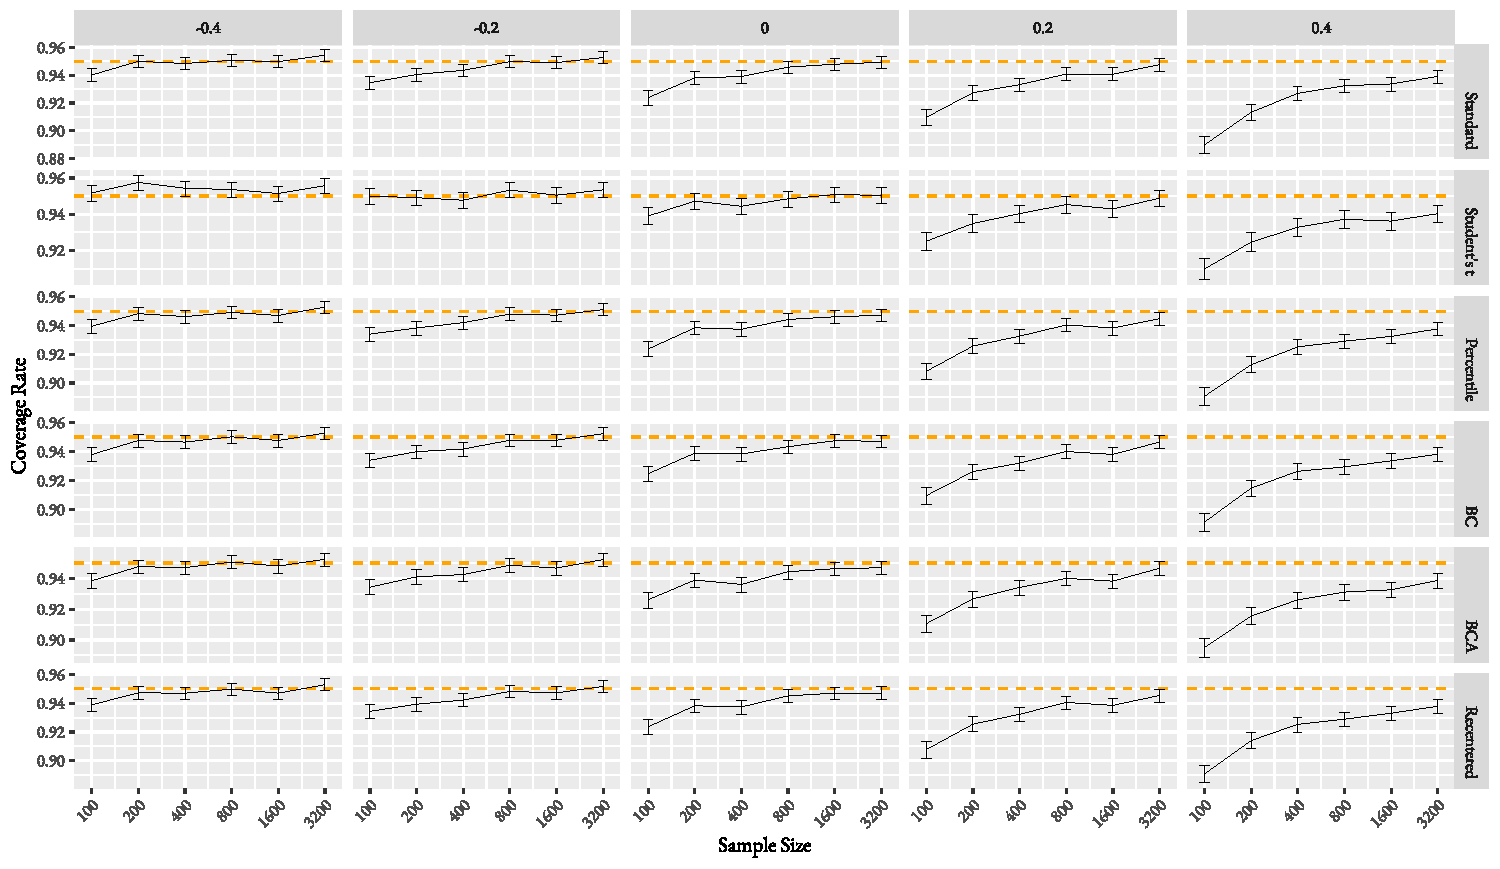
\includegraphics[width=\textwidth]{figures/plot_exp_mu_1}
  \caption{Empirical coverage rates of different 95\% block bootstrap CIs for
    the marginal mean $\mu$ of a stationary series with marginal unit exponential
    distribution obtained by transforming an AR(1) process with
    $\phi \in \{-0.4, 0.2, 0, 0.2, 0.4\}$ with series length
    $n \in \{100, 200, 400, 800, 1600, 3200\}$ based on 10,000 replicates of
    block bootstrap with $l = \lceil n^{1/3} \rceil$. 
    The error bars represent 95\% CIs of the real coverage rates.}
  \label{fig:exp_mu1}
\end{figure}


\begin{figure}[tbp]
  \centering
  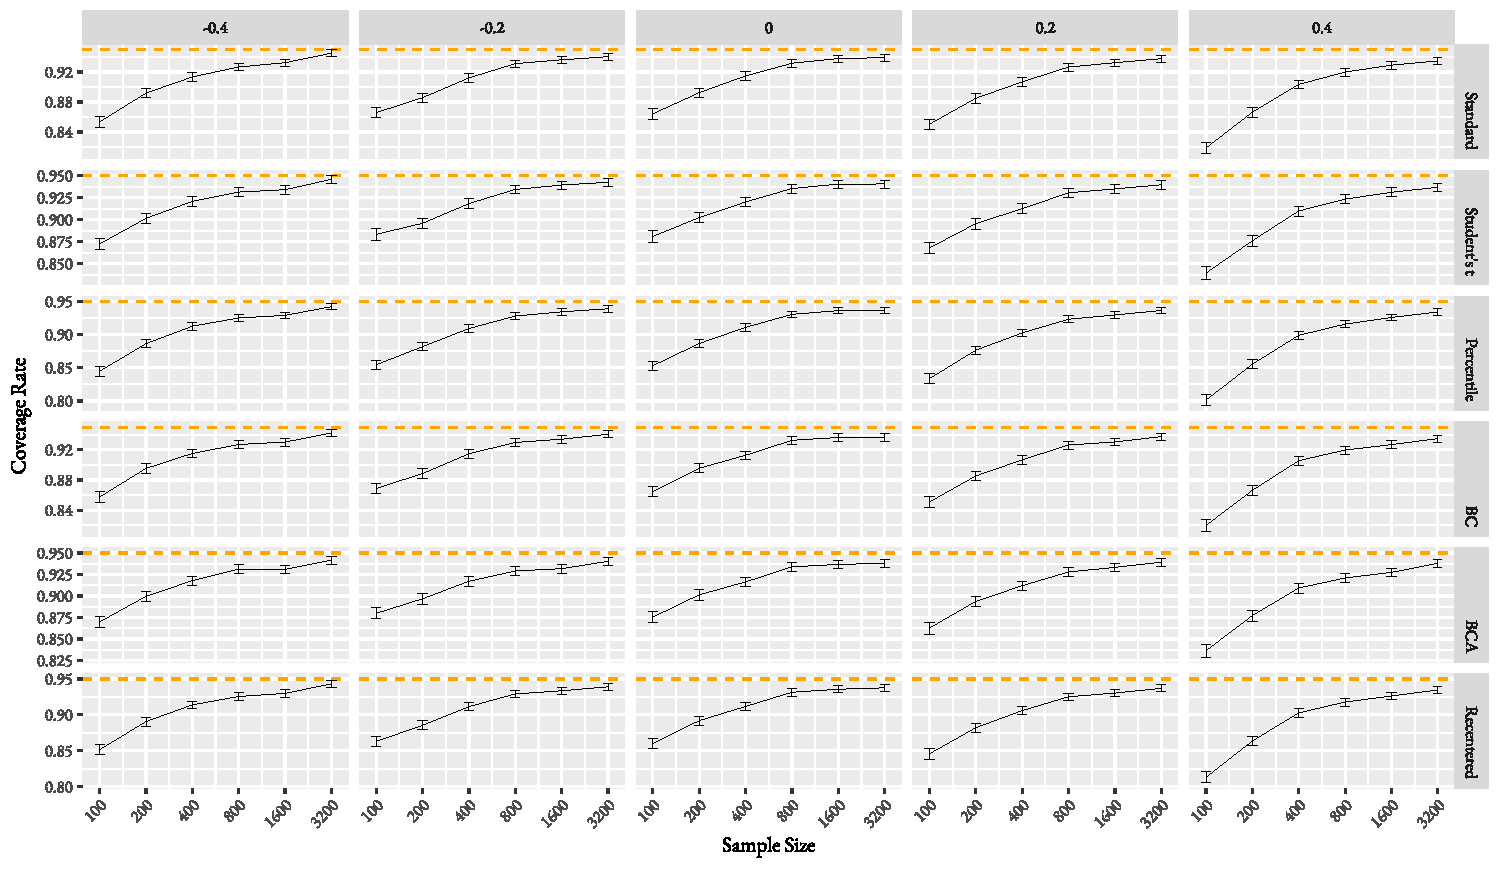
\includegraphics[width=\textwidth]{figures/plot_exp_sigma_1}
  \caption{Empirical coverage rates of different 95\% block bootstrap CIs for
    the marginal standard deviation $\sigma_w$ %\eds{$\sigma_w$?} \mc{addressed}
    of a stationary series with 
    marginal unit exponential distribution obtained by transforming an AR(1) process
    with $\phi \in \{-0.4, 0.2, 0, 0.2, 0.4\}$ with series length 
    $n \in \{100, 200, 400, 800, 1600, 3200\}$ based on 10,000 replicates 
    replicates of
    block bootstrap with $l = \lceil n^{1/3} \rceil$. 
    The error bars represent 95\% CIs of the real coverage rates.}
  \label{fig:exp_sigma1}
\end{figure}


\begin{figure}[tbp]
  \centering
  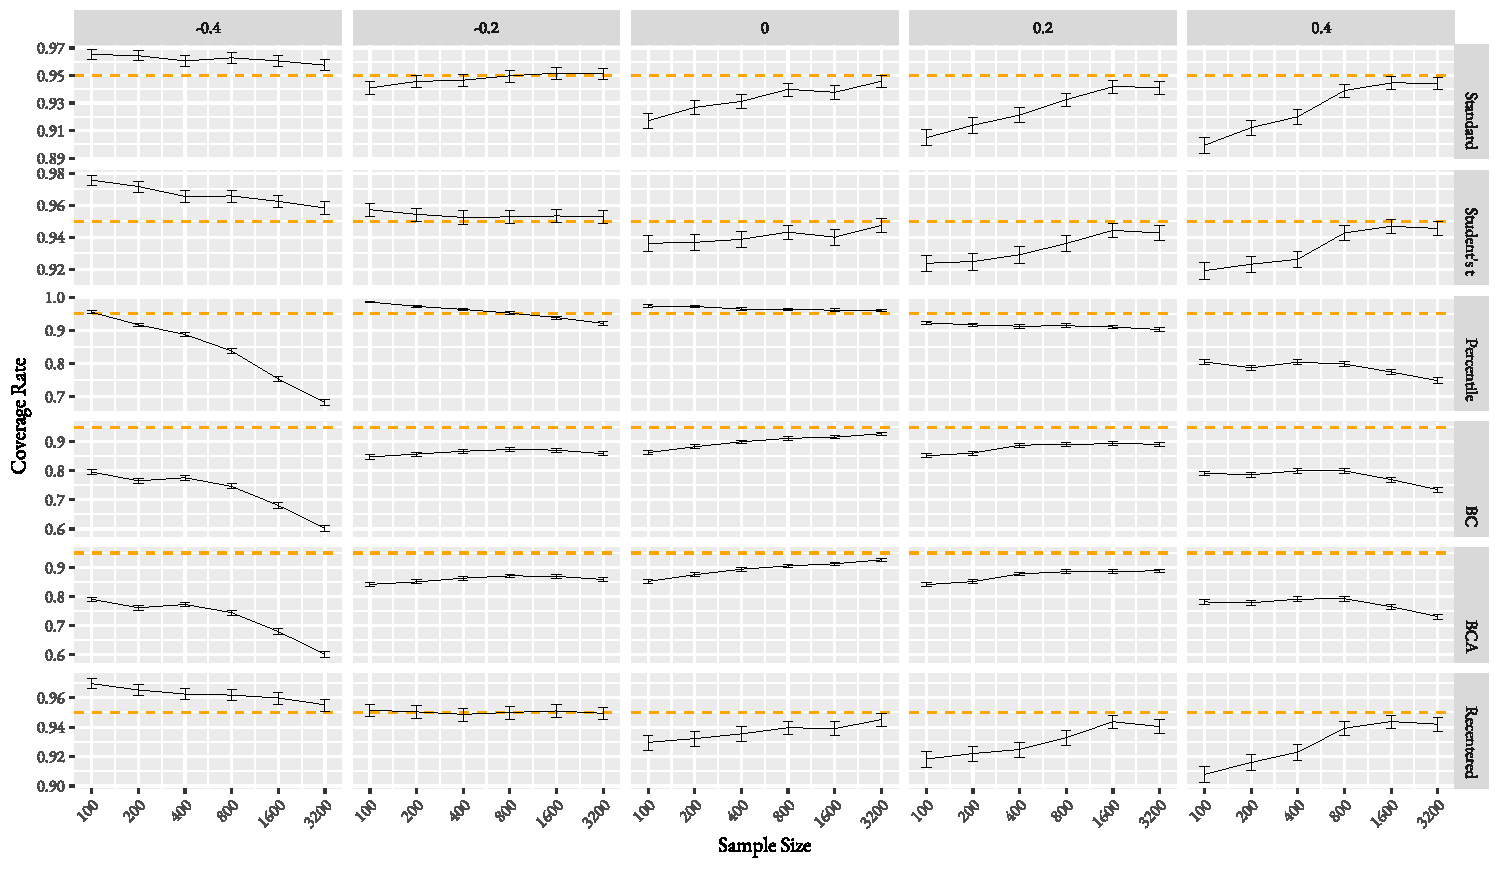
\includegraphics[width=\textwidth]{figures/plot_exp_phi_1}
  \caption{Empirical coverage rates of different 95\% block bootstrap CIs for 
    the first-order autocorrelation coefficient of a stationary series
    with marginal unit exponential distribution obtained by transforming an AR(1) 
    process with 
    $\phi \in \{-0.4, 0.2, 0, 0.2, 0.4\}$ with series length
    $n \in \{100, 200, 400, 800, 1600, 3200\}$ based on 10,000 replicates 
    replicates of
    block bootstrap with $l = \lceil n^{1/3} \rceil$. 
    The error bars represent 95\% CIs of the real coverage rates.}
  \label{fig:exp_phi1}
\end{figure}


\begin{figure}[tbp]
  \centering
  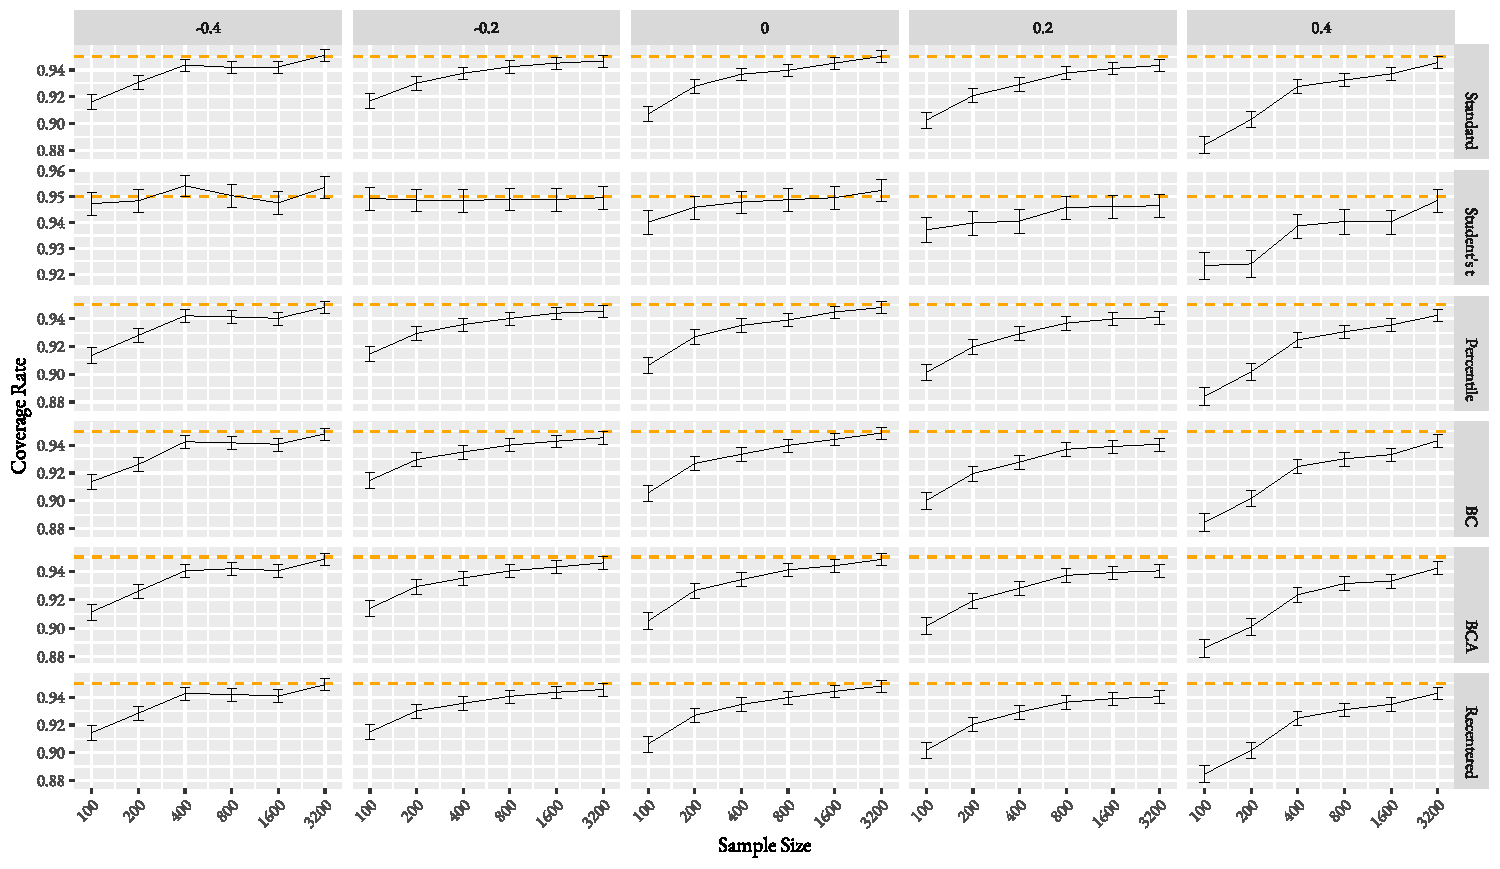
\includegraphics[width=\textwidth]{figures/plot_exp_mu_2}
  \caption{Empirical coverage rates of different 95\% block bootstrap CIs for
    the marginal mean $\mu$ of a stationary series with marginal unit exponential
    distribution obtained by transforming an AR(1) process with
    $\phi \in \{-0.4, 0.2, 0, 0.2, 0.4\}$ with series length
    $n \in \{100, 200, 400, 800, 1600, 3200\}$ based on 10,000 replicates of
    block bootstrap with $l = \lceil 2n^{1/3} \rceil$. 
    The error bars represent 95\% CIs of the real coverage rates.}
  \label{fig:exp_mu2}
\end{figure}


\begin{figure}[tbp]
  \centering
  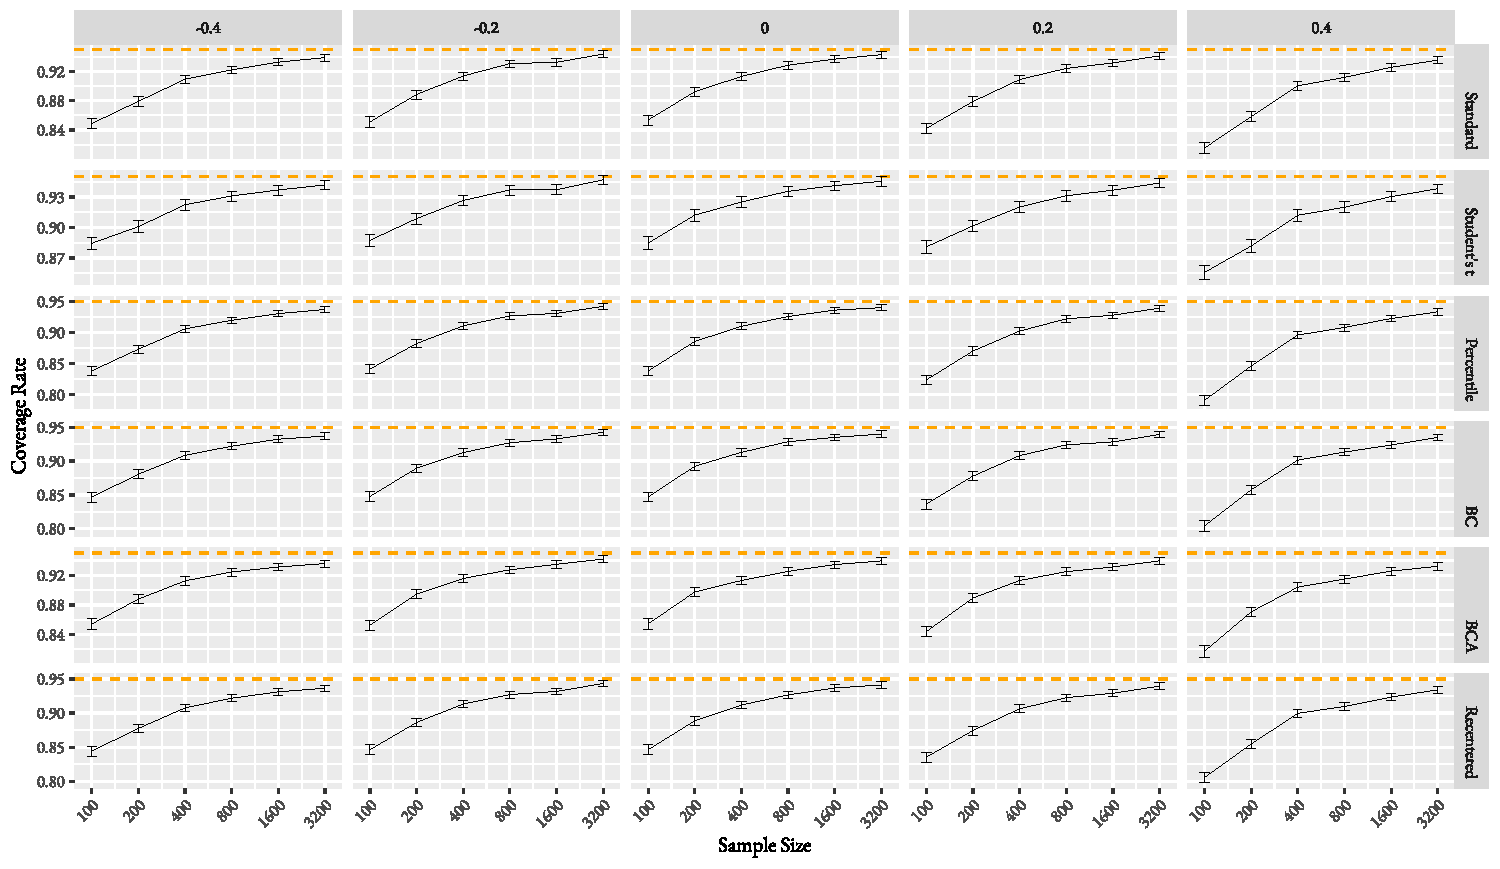
\includegraphics[width=\textwidth]{figures/plot_exp_sigma_2}
  \caption{Empirical coverage rates of different 95\% block bootstrap CIs for
    the marginal standard deviation $\sigma_w$ %\eds{$\sigma_w$?} \mc{addressed}
    of a stationary series with 
    marginal unit exponential distribution obtained by transforming an AR(1) process
    with $\phi \in \{-0.4, 0.2, 0, 0.2, 0.4\}$ with series length 
    $n \in \{100, 200, 400, 800, 1600, 3200\}$ based on 10,000 replicates 
    replicates of
    block bootstrap with $l = \lceil 2n^{1/3} \rceil$. 
    The error bars represent 95\% CIs of the real coverage rates.}
  \label{fig:exp_sigma2}
\end{figure}


\begin{figure}[tbp]
  \centering
  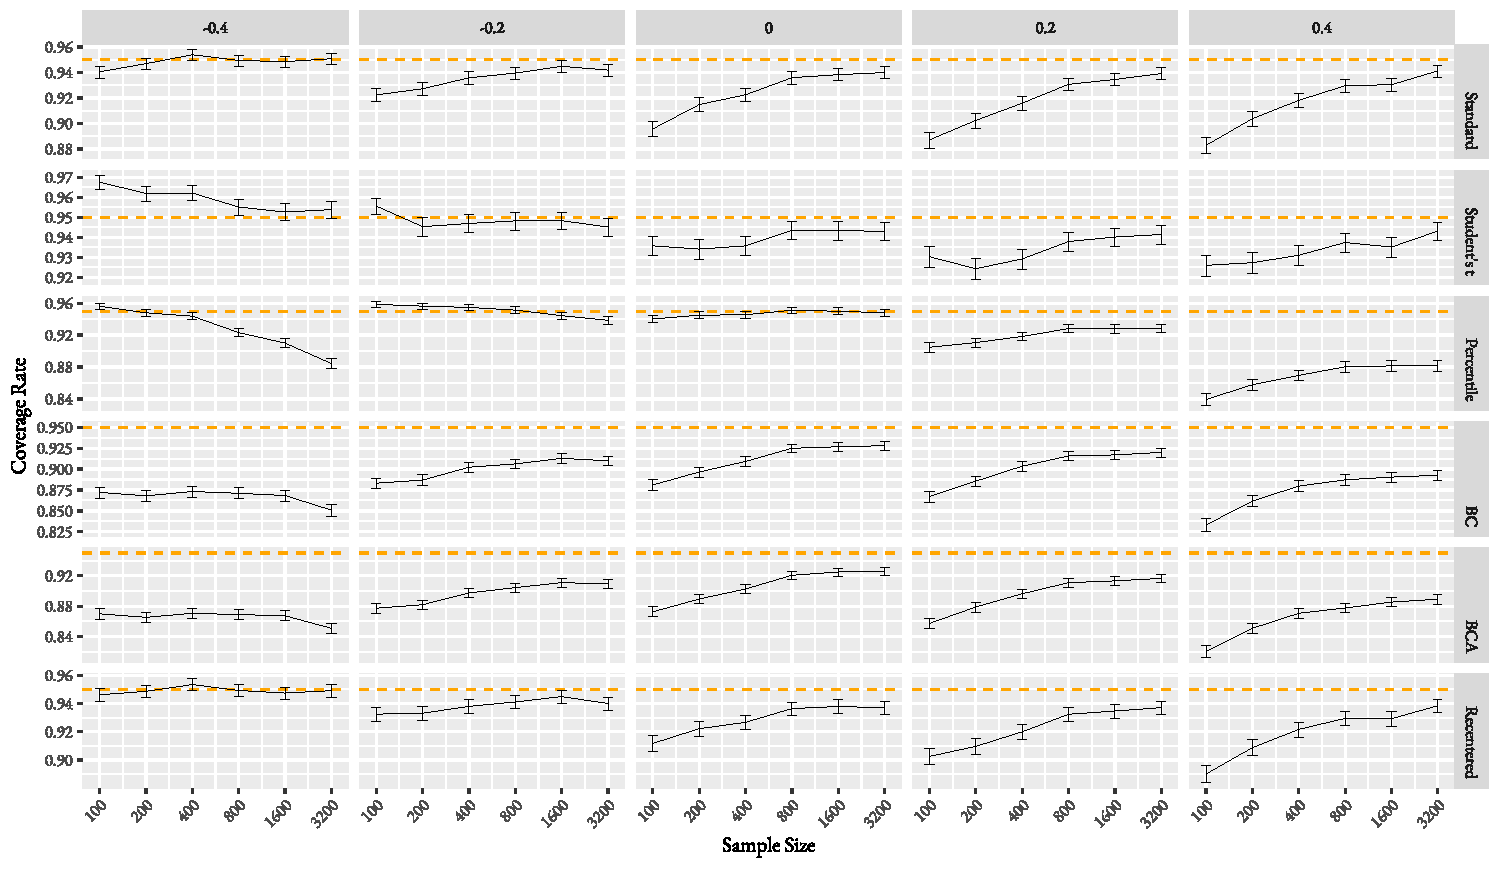
\includegraphics[width=\textwidth]{figures/plot_exp_phi_2}
  \caption{Empirical coverage rates of different 95\% block bootstrap CIs for 
    the first-order autocorrelation coefficient of a stationary series
    with marginal unit exponential distribution obtained by transforming an AR(1) 
    process with 
    $\phi \in \{-0.4, 0.2, 0, 0.2, 0.4\}$ with series length
    $n \in \{100, 200, 400, 800, 1600, 3200\}$ based on 10,000 replicates 
    replicates of
    block bootstrap with $l = \lceil 2n^{1/3} \rceil$. 
    The error bars represent 95\% CIs of the real coverage rates.}
  \label{fig:exp_phi2}
\end{figure}

\begin{figure}[tbp]
  \centering
  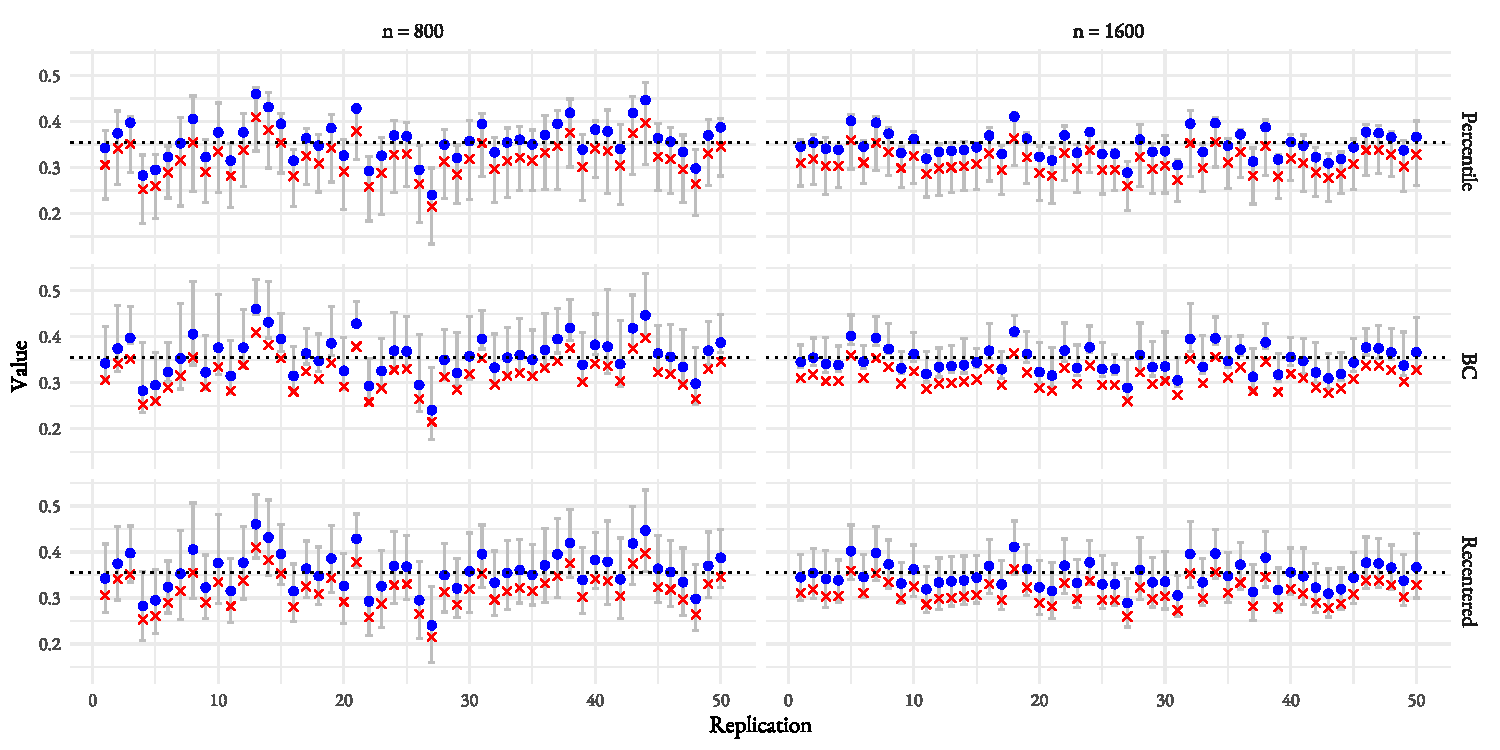
\includegraphics[width=\textwidth]{figures/exp_phi_intervals}
  \caption{50 replicate percentile, BC, and recentered percentile CIs for the
    lag-1 autocorrelation coefficient 0.355 ($\phi = 0.4$)
    of a stationary series with marginal exponential distribution
    obtained by transforming an AR(1) process with $\phi = 0.4$ with
    sample size $n \in \{800, 1600\}$ ($l = \lceil n^{1/3} \rceil$). For 
    each replicate, the lower and upper bounds of the CIs are displayed, as well 
    as $\hat\theta_n$ (blue circle) and $\bar\theta_n^{B}$ (red cross).}
  \label{fig:eri}
\end{figure}


For an exponential marginal distribution, the empirical coverage rates for 
$\mu$, $\sigma_w$, %\eds{define $\sigma_w$} 
%\mc{added definitions for $\mu$ and $\sigma_w$ in the above paragraph} 
and 
the lag-1 autocorrelation coefficient, %\mc{replaced $\phi$ here, as I understand
%it, we are not using $\phi$ in reference to the temporal dependence of the 
%exponentially distributed series?}, 
as well as 95\%
confidence intervals of the real coverage are displayed in 
\textbf{Figures~\ref{fig:exp_mu1}--\ref{fig:exp_phi2}}. 
Additionally, a set of 50 CIs are displayed for each of the percentile, 
BC, and recentered percentile approaches for exponentially distributed
samples of $n \in \{800, 1600\}$ with lag-1 autocorrelation coefficient 0.355
($\phi = 0.4$) in Figure~\ref{fig:eri}.


It appears that a greater sample size is generally required for the bootstrap
CIs to cover the mean and standard deviation parameters in the exponential
margin case than in the normal margin case. However, the trends and patterns
discussed in the main text regarding the performance of various methods and
diverse parameters remain consistent. For example, Student's $t$ confidence
intervals still exhibit higher coverage rates in comparison to alternative
methods. Performance continues to be more favorable when temporal dependence is
negative rather than positive. Altering the block size results in the same 
changes in performance of different CIs. Of particular significance, the 
percentile, BC,
and BCA confidence intervals still display a decline in coverage accuracy for
the lag-1 autocorrelation coefficient as sample size increases as demonstrated
in Figure~\ref{fig:eri}. Both the percentile and BC intervals persist in
manifesting the same bias issue. On the other hand, the recentered percentile
confidence interval continues to be effective in estimating the temporal 
dependence %\mc{replaced $\phi$ again here} 
due to the
inherent unbiasedness of the original point estimator. In sum, the findings for
series that are marginally exponentially distributed closely mirror those
attained for series that are marginally normally distributed.


\begin{comment}
10.   Why did the authors choose to only go as high as 0.4 (and as low as -0.4) 
for the autocorrelation parameter?  I would think that these correlations near 1 
(or -1) would be some of the more interesting cases to study, but they are 
completely ignored here.  Can the authors justify their choice to leave it out 
of this study?
\end{comment}

Thank you for the comment. We have now included this comment in the Design 
subsection:

We only
used serial dependences as strong as 0.4, because we only seek to 
establish the 
general trend as the strength of the autocorrelation 
increases, and how it varies depending on the sign of the autocorrelation and 
the parameter of interest.

\begin{comment}
11.    Last paragraph: The authors mention the “ABC and bootstrap-t intervals”.  
They do not give a citation for these intervals.   Add a citation. 
\end{comment}

We apologize for the omission. These intervals are discussed in 
\citep{efron1993introduction}. A citation is now provided in the last paragraph.



\begin{comment}
12.    The last line of the manuscript offers one line about the drawbacks of 
the block bootstrap almost as an afterthought.  I think a discussion of the 
drawbacks should be expanded and added to the introduction as this is an 
important point that isn’t mentioned at all until the literal last line. 
\end{comment}

Thank you for the comment. We have included this discussion of problems 
with block bootstrap in the introduction:

\citet{lahiri1999theoretical} finds that moving block bootstrap has better 
performance than non-overlapping block bootstrap. Additionally, moving block 
bootstrap with nonrandom
block sizes results in lower mean-squared errors than moving block bootstrap
with random block sizes. \citet{buhlmann1999block} notes that a drawback of 
block bootstrap is that it heavily depends on block size, which has to be chosen
by the user of the method.
Even when using the appropriate settings, as noted by
\citet{buhlmann2002bootstraps} observes some general drawbacks of block 
bootstrap --- with respect to how reasonably it imitates the data-generating 
process. In addition, although block bootstrap is primarily used for stationary 
time series, it can be outperformed by other bootstrap schemes for linear time
series and categorical processes. Still, \citet{buhlmann2002bootstraps}
emphasizes that a significant advantage of block bootstrap is its simplicity.
To be more specific, the resampling step of block bootstrap is not 
computationally more difficult than the resampling step of basic bootstrap.
Furthermore, block bootstrap performs better than local bootstrap in terms of
mimicking dependence structures.

\eds{If we include all these drawbacks in the intro, we need to also provide 
some good features of block bootstrap as well, otherwise, why do we care about 
their CI performance?}
\mc{addressed}

We also added this comment in the Discussion section:

We discussed some
drawbacks of block bootstrap in the introduction, which could motivate a similar
simulation study for alternatives to block bootstrap, such 
as AR-Sieve bootstrap, \citep{kreiss1992bootstrap} which 
\citet{buhlmann2002bootstraps} finds to be the best for linear time series. 

We are indebted to the reviewers for pointing out these vital discussion areas,
which have not only enriched the current paper but also charted a clear course
for our subsequent research endeavors.


\bibliographystyle{chicago}
\bibliography{citations}


\end{document}
